% !TEX encoding = UTF-8 Unicode
\documentclass{beamer}

\usepackage{amsmath}
\usepackage[english,brazil]{babel}
\usepackage[utf8]{inputenc}
\usepackage{graphicx}
\usepackage{url,color, colortbl}
\usepackage{subfigure}
\usepackage{makeidx} 
\usepackage{subfloat}
\usepackage{float}
\usepackage{listings}  
\usepackage{wrapfig} 
\usepackage{verbatim}  
\usepackage{caption} 
\usepackage{algorithm,algorithmic}
\usepackage{beamerthemesplit}
\usepackage{xcolor}

\definecolor{cl-programado}{rgb}{1,0.6,0}
\definecolor{cl-realizado}{rgb}{0,0.7,0.32}
\definecolor{cl-atrasado}{rgb}{0.75,0,0}
\definecolor{cl-cabecalho}{rgb}{0.3,0.5,0.75}
\definecolor{cl-impar}{rgb}{0.81, 0.85, 0.91}
\definecolor{cl-par}{rgb}{0.91, 0.93, 0.87} 
 
 
%\newcommand{\newblock}{}
%\usepackage[portugues,algoruled,longend]{algorithm2e}  
%-----   Themes ------%
% \usetheme{Madrid}
% \usetheme{Warsaw}
% \usetheme{Boadilla}
 \usetheme{CambridgeUS}
% \usetheme{Montpellier}
% \usetheme{Hannover}
% \usetheme{Dresden}

% \definecolor{verdeescuro}{rgb}{0.539,0.601,0.42}
\definecolor{cor}{rgb}{0.0,0.0,0.5}  
%\definecolor{verde}{rgb}{0.55,0.78,0.25} 
% ------------------------------------------------------------------ %
% Deixando o tema mais verde. Comente a linha abaixo se nao gostar %
\setbeamercolor{structure}{fg=cor}
% ------------------------------------------------------------------ %
% Deixando o verde mais claro para combinar com o logo do IFET
% Descomente as linhas abaixo
% \setbeamercolor{structure}{fg=verde}
% \setbeamercolor{title}{fg=black,bg=verde!80!black}
% \setbeamercolor{frametitle}{fg=black,bg=verde!25}
% \setbeamercolor{block body}{fg=black,bg=verde!15}
% \setbeamercolor{block title}{fg=white,bg=verdeescuro}
% ------------------------------------------------------------------ %
\linespread{1}
\beamertemplatenavigationsymbolsempty

\title[Proposta]{Sistemas de Defesa: Uma abordagem para desvios de obstáculos no auxílio do controle de um quadricóptero em tempo real}

\author[Bruno Giovanini]{Bruno da Silva Giovanini
\\   
\vspace{1cm}
$\mbox{Paulo F.F. Rosa}^1$\\
(Orientador)
%\\\footnotesize{angonesealberto@gmail.com, rpaulo@ime.eb.br}}
% \\ Eduardo Krempser  
% \\\footnotesize{krempser@lncc.br}}
}
\institute[IME]{
	\inst{1}
		Instituto Militar de Engenharia - IME\\
		Laboratório de Robótica e Inteligência Computacional\\ 
		Programa de Pós-graduação em Engenharia de Defesa \\ 		
	
}


\date{\today}

\begin{document}




\begin{frame}
 \titlepage	
\end{frame}

% ------------ Inicio do documento ---------------%
%\section*{Sum�rio}
\begin{frame}
	\frametitle{Sumário}  
	\tableofcontents
\end{frame}
% -------------------------------------------------%
\section{Introdução}

\begin{frame}
	\frametitle{Sumário}
	\tableofcontents[currentsection]
\end{frame}


\begin{frame}[allowframebreaks]
 	\pgfdeclareimage[width=1.0cm]{logo}{img/ime.png}
	\frametitle{\insertsection}
	\begin{itemize}
	    \item Crescente utilização para missões civis e militares
	     
	    \item Voos em ambientes fechados e restritos
	     
	    \item Risco de colisão com equipamentos críticos e sensíveis
	    
	    \item Difícil controle e manuseio
	    
	    
	\framebreak
		\vspace{2cm}
		
		\begin{figure}
			\centering
			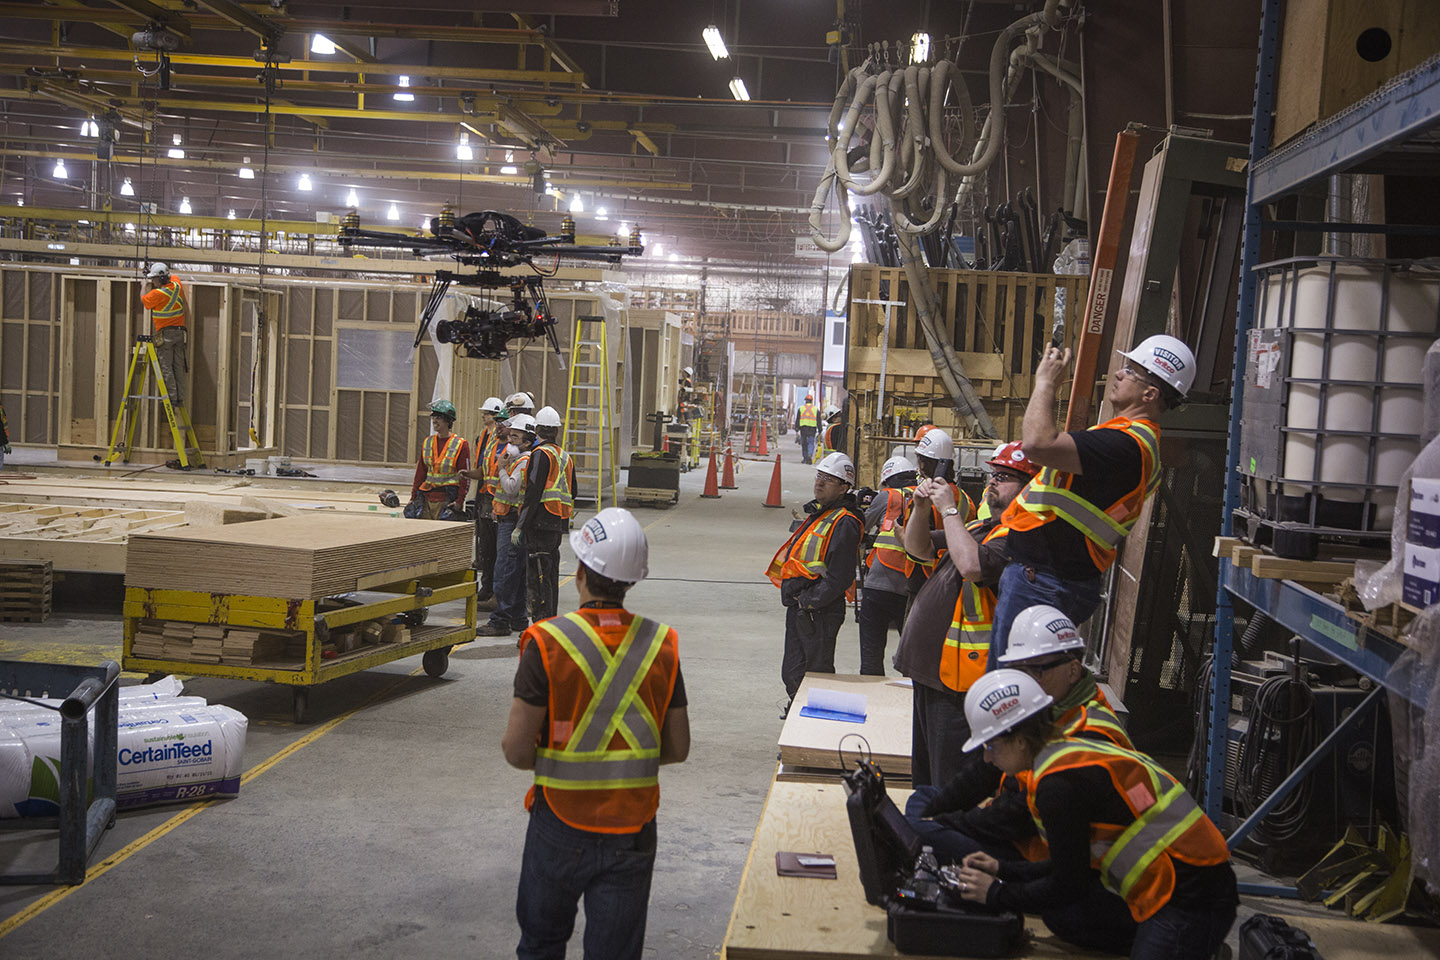
\includegraphics[keepaspectratio = true,
			width=0.7\textwidth]{img/filmagem_drone.jpg}
			\label{fig:obr2013}
			\caption{Filmagem \textit{indoor}}
		\end{figure}
			
	\framebreak
		\vspace{2cm}
		
		\begin{figure}
			\centering
			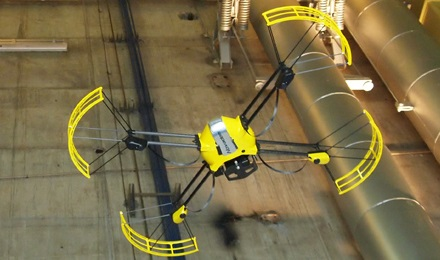
\includegraphics[keepaspectratio = true,
			width=0.7\textwidth]{img/Inspection-Drone.jpg}
			\label{fig:obr2013}
			\caption{Inspeção de equipamentos sensíveis}
		\end{figure}
			
	\end{itemize}	
\end{frame}

\subsection*{Objetivo}

\begin{frame}
	\frametitle{Objetivo}	
	
	\begin{itemize}
		\item Evitar colisões de um quadricóptero, estimando constantemente a trajetória futura do veículo, com base na sua dinâmica, seu estado atual, o \textit{input} de controle corrente e a distância para os obstáculos, medida através de sensores ultrassônicos embarcados
		 
		
		 
		 \item Maior segurança no voo desta plataforma em ambientes restritos
	\end{itemize} 
	 	
\end{frame}

% -------------------------------------------------%

\section{Tópicos tutorias}

\begin{frame}
	\frametitle{Sumário}
	\tableofcontents[currentsection]
\end{frame}

\subsection*{O quadricóptero}
\begin{frame}
  	
	\frametitle{O quadricóptero - A Plataforma}
	
	\begin{itemize}
	
	\item Veículo voador com quatro rotores com decolagem e aterrissagem vertical \cite{Salih2010}
		
	\begin{figure}
		\centering
		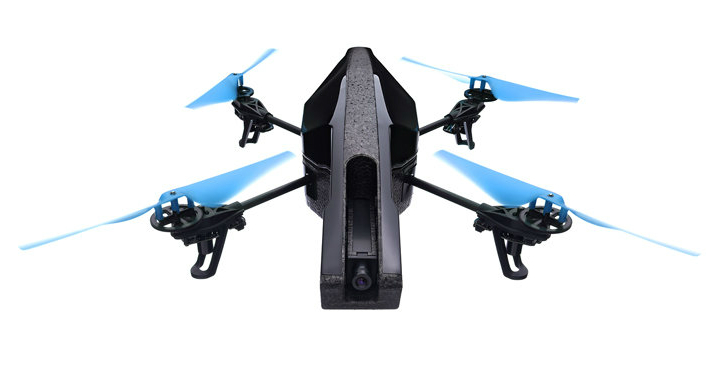
\includegraphics[keepaspectratio = true,
		width=0.7\textwidth]{img/parrot_drone.jpg}
		\caption{Plataforma Parrot Ardrone 2.0. Fonte \cite{ardrone}}
		\label{fig:quad}
	\end{figure}
		
	\end{itemize}
	
\end{frame}

\begin{frame}[allowframebreaks]
	
	\frametitle{O quadricóptero - Dinâmica de Voo}
	
	\begin{itemize}
		
		\item Seis graus de liberdade e quatro atuadores
				
		\item Três são movimentos lineares ($x$,$y$,$z$) e três são angulares ($\phi$,$\theta$,$\psi$)
						
		\item  Sistema \textit{underactuated}, movimentos (x,y) dependentes dos movimentos ($\phi$,$\theta$)
				
		\item Objetivo é manter a estabilidade do eixo central controlando quatro motores independentes eletronicamente
		
	\framebreak	
		
		\begin{figure}
			\centering
			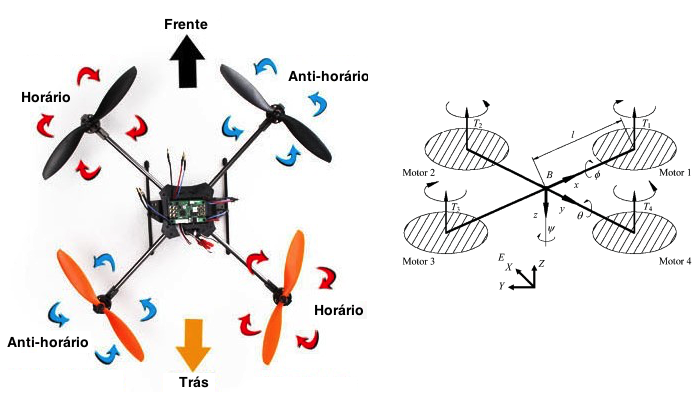
\includegraphics[keepaspectratio = true,
			width=0.6\textwidth]{img/diagrama_quadricoptero.png}
			\caption{Estrutura e orientação dos motores (a), as forças e momentos atuando no quadricóptero (b) e os movimentos gerados a partir das variações de velocidades dos motores (c). Fontes \cite{quadblog}, \cite{Mian2008} e \cite{Domingues2009}.}
			\label{fig:diag quad}
		\end{figure}
	
	\end{itemize}	
	
\end{frame}	 

\subsection*{Sistemas embarcados para navegação}
\begin{frame}
	
	\frametitle{Sistemas embarcados para navegação}
	
	\begin{itemize}

	\item Obtenção de informações sobre a posição, velocidade e atitude de um veículo com relação a um dado referencial	
	
	\item Fornecidas por sensores inerciais: acelerômetros e giroscópios
	
	\item Magnetômetros incluídos melhoram a medida da atitude do veiculo	
	
	\end{itemize}
	
\end{frame}	
\begin{frame}[allowframebreaks]
	\frametitle{IMU}
	
	\begin{itemize}
		
		\item Componente eletrônico onde estão montados os sensores. 
		
		\item Três acelerômetros: aceleração linear (x,y,z)
		
		\item Três giroscópios: velocidade angular ($\phi$,$\theta$,$\psi$)
	
	    \vspace{0.5cm}
	
		\begin{figure}[h]
			\centering
			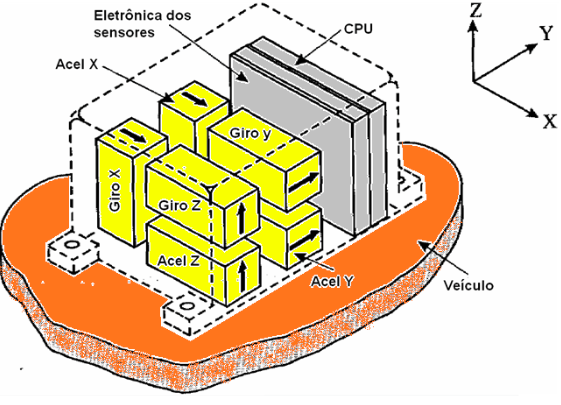
\includegraphics[keepaspectratio = true,
			width=0.65\textwidth]{img/imuStrap.png}
			\caption{Estrutura do Sistema de Navegação acoplada ao veículo (esquerda) e os movimentos gerados no quadricóptero (direita). Fonte \cite{Adalberto2009}}
			\label{fig:imuStrap}
		\end{figure}
		
	\framebreak
	
		\begin{figure}
			\centering
			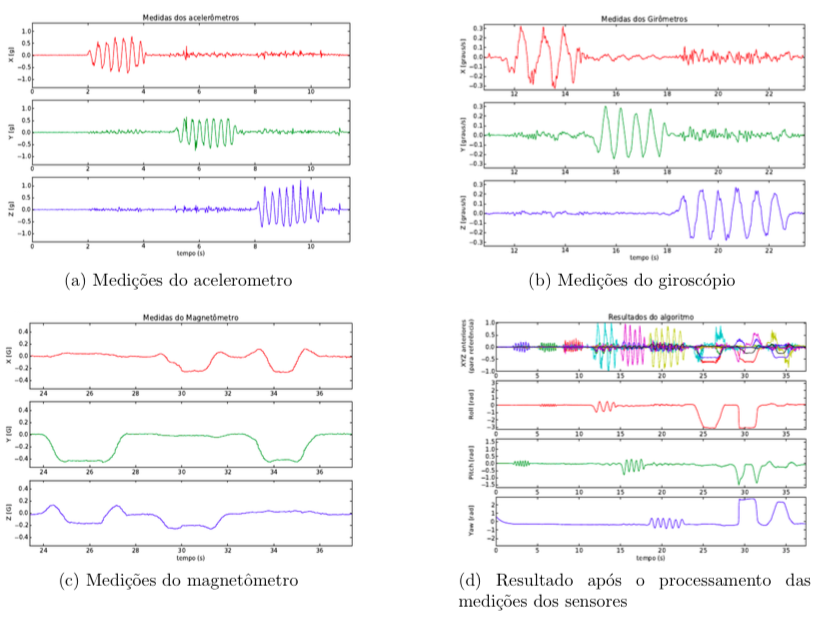
\includegraphics[keepaspectratio = true,
			width=0.63\textwidth]{img/imu_VANTIME.png}
			\caption{Gráfico das medições dos sensores inerciais da IMU do VANT-IME. Fonte \cite{Paixao2011}}
			\label{fig:imuVANTIME}
		\end{figure}
	
	\end{itemize}
\end{frame}	

\subsection*{Controle PID e quadricópteros}
\begin{frame}[allowframebreaks]
	
	\frametitle{Controle PID}
	\begin{itemize}
	
		\item Método comum para controle de robôs
		
		\item Controle fechado que reage a mudanças no ambiente captadas por sensores
		
		\item Três parâmetros constantes: Proporcional (P), Integral (I) e Derivativo (D)
		
	\framebreak
	
		\item Proporcional (P)
			\begin{itemize}
				\item É tipicamente o erro. 
				\item Fórmula: $A - B$, onde $A$ é a posição atual e $B$ é onde deveria estar 	
			\end{itemize}
			
		\item Integral (I)
		\begin{itemize}
			\item É o acúmulo dos erros passados no tempo. 
			\item Fórmula: $A/t_1 + B/t_2 + C/t_3$, sendo $A$ o erro em $t_1$, $B$ em $t_2$ e $C$ em $t_3$ 	
		\end{itemize}	
		
		\item Derivativo (D)
		\begin{itemize}
			\item É a mudança do erro no tempo. 
			\item Fórmula: $(A-B)/t$, sendo $A$ o erro inicial e $B$ o erro depois do tempo $t$ 	
		\end{itemize}	
		
	\framebreak
	
		\item Cada parâmetro tem seu ganho $K$ associado
		
		\item Soma ponderada: $P*K_p + I*K_i + D*K_d$
		
		\vspace{0.6cm}
		\begin{figure}[h]
			\centering
			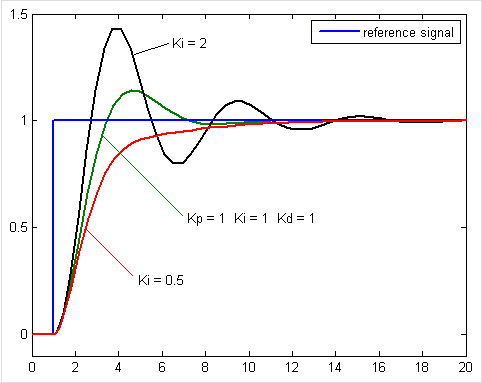
\includegraphics[keepaspectratio = true,
			width=0.4\textwidth]{img/ganho_PID.png}
			\caption{Desempenho do sistema para diferentes ganhos $K_p$, $K_i$ e $K_d$. Fonte \cite{Kingdom}}
			\label{fig:ganhoPID}
		\end{figure}	
	
	\end{itemize}
	
\end{frame}	

\begin{frame}[allowframebreaks]
	
	\frametitle{PID para quadricópteros}
	
	\begin{figure}[h]
		\centering
		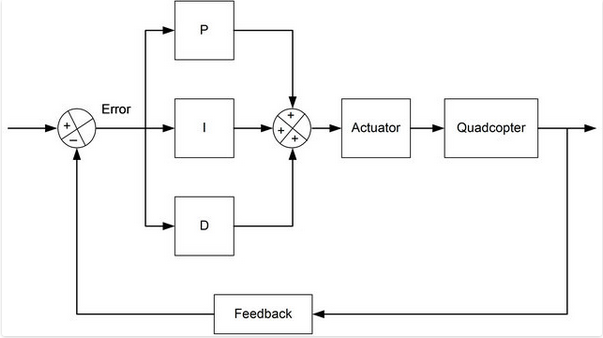
\includegraphics[keepaspectratio = true,
		width=0.8\textwidth]{img/PID_quad_geral.png}
		\caption{Controle PID de um quadricóptero. Fonte \cite{Liang}}
		\label{fig:PIDquad}
	\end{figure}
	
	\framebreak
	
	\begin{figure}[h]
		\centering
		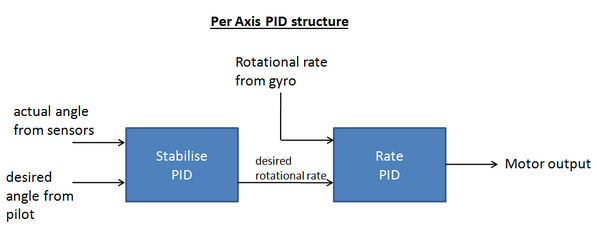
\includegraphics[keepaspectratio = true,
		width=0.7\textwidth]{img/PID_quad_axis.png}
		\caption{Controle PID por eixo. Fonte \cite{Liang}}
		\label{fig:PIDaxis}
	\end{figure}
	
	
\end{frame}	


\section{O Problema: Segurança em voo para quadricóptero}

\begin{frame}
	\frametitle{Sumário}
	\tableofcontents[currentsection]
\end{frame}

\begin{frame}[allowframebreaks]
	\frametitle{O Problema: Segurança em voo para quadricóptero}
	
	\begin{itemize}
		
		\item Auxíliar o controle da plataforma com base na dinâmica, estado  atual, controle corrente e distância para obstáculos
		
		\item Dado $\mathcal{X} \subset \mathbb{R}^{n}$ o espaço de estados do robô, $\mathcal{U} \subset \mathbb{R}^{n}$ o espaço do \textit{input} de controle, $t$ o tempo, $\mathbf{x}(t)$ o estado do robô no tempo $t$ e $\mathbf{u}(t)$ o \textit{input} de operação no tempo $t$.A dinâmica do robô é uma função em $\mathbf{f} \in \mathcal{X} \times \mathcal{U} \times \mathbb{R} \rightarrow \mathbb{R}^{n}$ e é dada pela relação \ref{eq:equacaoDinProb}:
		
		\begin{equation}
		\centering
		\dot{\mathbf{x}} = \mathbf{f}(\mathbf{x}(t),\mathbf{u}(t),t)  
		\label{eq:equacaoDinProb}
		\end{equation}
		
		\item Com $\mathbf{x_0} = \mathbf{x}(0)$ e uma constante de \textit{input} de operação $\mathbf{u}$, o estado do robô será:
		
		\begin{equation}
		\centering
		\mathbf{x} = \mathbf{g}(\mathbf{x},\mathbf{u},t)  
		\label{eq:equacaoPosProb}
		\end{equation}
		
		onde $\mathbf{g} \in \mathcal{X} \times \mathcal{U} \times \mathbb{R} \rightarrow \mathcal{X}$ é a solução da equação diferencial \ref{eq:equacaoDinProb}				
		
	\framebreak
	
		\item Obstáculos restringem as posições possíveis do robô
		
		\item Sendo $\mathcal{O} \subset \mathbb{R}^3$, a subárea do espaço $\mathbb{R}^n$ de movimentos possíveis do robô ocupadas por obstáculos e as regiões escondidas por eles quando vistas robô e $\mathcal{R}(x)$, a subárea ocupada pelo robô no estado $x \in \mathcal{X}$
			
		\item O Problema: Definir a menor variação de controle $\Delta\mathbf{u} \in \mathcal{U}$ necessária para evitar colisão na janela de tempo $t \in [0,\tau]$, onde $\tau$ é um horizonte de tempo já definido:
		
		\begin{equation}
		\begin{aligned}
		\text{min: }& \Delta\mathbf{u} \\
		\text{Sujeito a: }& \forall t \in [0,\tau], \mathcal{R}(\mathbf{g}(\mathbf{x}, \mathbf{u}+\Delta\mathbf{u}, t)) \cap \mathcal{O} = \emptyset
		\end{aligned}
		\label{eq:equacaoProb}
		\end{equation}
		
		
	\end{itemize}	 
\end{frame}


\section{Metodologia}

\begin{frame}
	\frametitle{Sumário}
	\tableofcontents[currentsection]
\end{frame}

\begin{frame}[allowframebreaks]
	
	\frametitle{Metodologia}
	
	\begin{itemize}
	
		\item Divisão em etapas
		
		\begin{figure}[h]
			\centering
			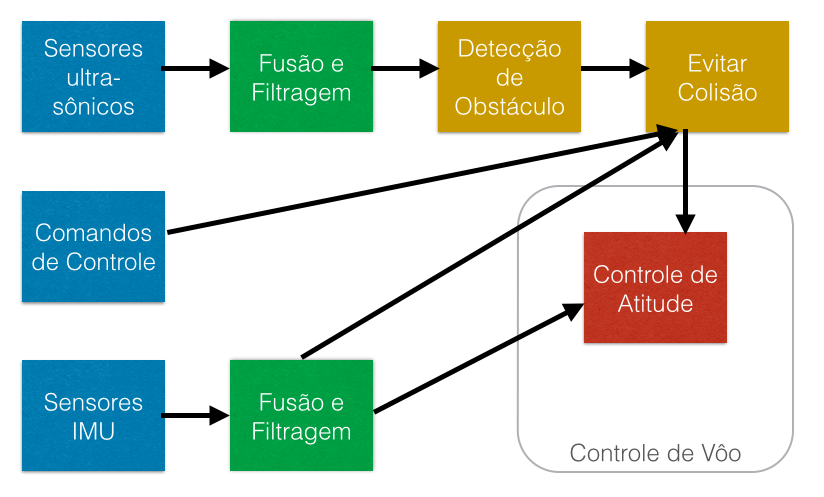
\includegraphics[keepaspectratio = true,
			width=0.7\textwidth]{img/etapasMetodo.png}
			\caption{Etapas do método}
			\label{fig:etapasMetodo}
		\end{figure}
		
	\framebreak
	
		\item Componentes necessários
		\begin{itemize}	
			
			\item Plataforma de voo (quadricóptero) com interface de comunicação e SDK código aberto
			
			\item Sensores ultrassônicos
			
			\item \textit{Conputer on module} para embarque na plataforma: Raspberry PI
				
		\end{itemize}
		
		\item Software necessário
		\begin{itemize}	
			
			\item Matlab com pacote Simulink
			
			\item Kit de desenvolvimento para quadricópteros do Matlab Simulink
			
			\item Raspberry Pi Support from MATLAB
			
		\end{itemize}
	
	\framebreak	
		
		\item Estratégia de implementação
		
		\begin{figure}[h]
			\centering
			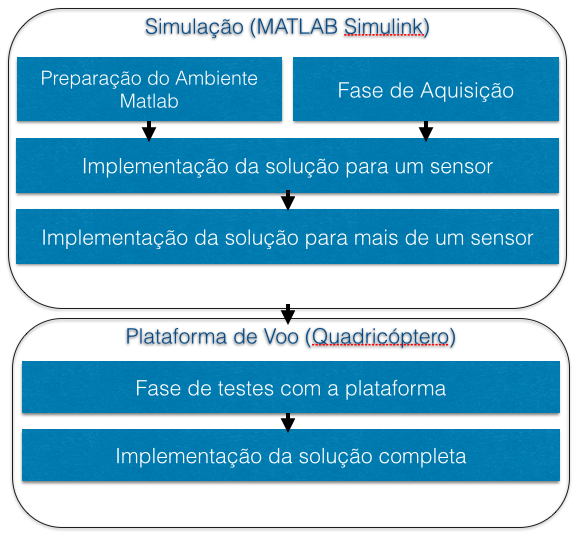
\includegraphics[keepaspectratio = true,
			width=0.5\textwidth]{img/fluxo.png}
			\caption{Estratégia de implementação}
			\label{fig:Fluxo}
		\end{figure}
			
	\end{itemize}	 
	
\end{frame}


\section{Cronograma}

\begin{frame}
	\frametitle{Sumário}
	\tableofcontents[currentsection]
\end{frame}

\begin{frame}
	
	\frametitle{Cronograma}
	
	\begin{figure}[h]
		\centering
		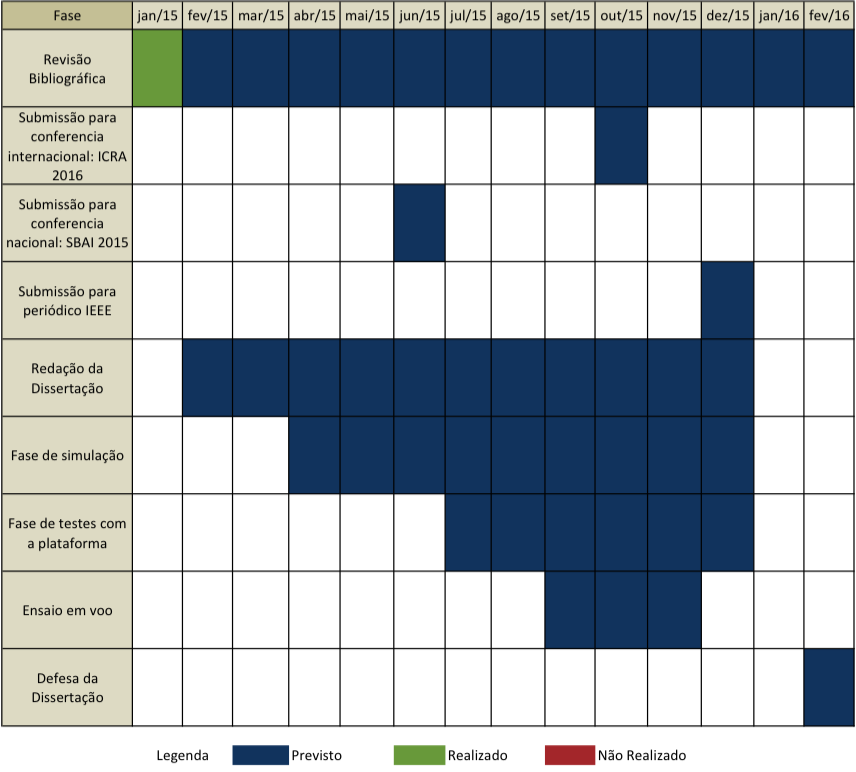
\includegraphics[keepaspectratio = true,
		width=0.63\textwidth]{img/cronograma.png}
		\caption{Cronograma físico.}
		\label{fig:cronograma}
	\end{figure}
	
\end{frame}	

\section{Viabilidade da proposta}

\begin{frame}
	\frametitle{Sumário}
	\tableofcontents[currentsection]
\end{frame}

\begin{frame}
	
	\frametitle{Viabilidade da proposta}
	
	\begin{itemize}	
		
		\item  Quatro quadricópteros com 45cm de diâmetro
		
		\item Dois Raspberry PI modelo B com processador de 700MHz, 512MB de memória
		
		\item Sensores ultrassónicos
		
		\item Matlab R2013a com Simulink
		
	\end{itemize}	
	
	
\end{frame}	

\section{Resultados esperados}

\begin{frame}
	\frametitle{Sumário}
	\tableofcontents[currentsection]
\end{frame}

\begin{frame}
	
	\frametitle{Resultados esperados}
	
	\begin{itemize}	
		
		\item  Foram elaboradas três missões
	\end{itemize}	
		\begin{columns}[T] % contents are top vertically aligned
			\begin{column}[T]{3cm} % each column can also be its own environment
				\begin{figure}
					\centering
					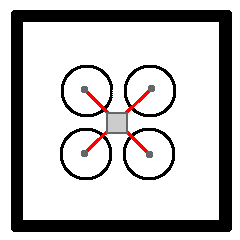
\includegraphics[keepaspectratio = true,
					width=1.0\textwidth]{img/missao1.png}
					\caption{Missão 1. Veículo cercado e estabilizado}
					\label{fig:missao1}
				\end{figure}
			\end{column}
			\begin{column}[T]{3cm} % alternative top-align that's better for graphics
				\begin{figure}
					\centering
					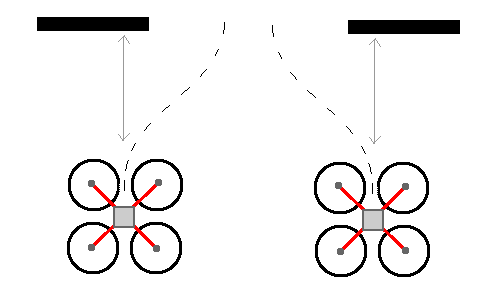
\includegraphics[keepaspectratio = true,
					width=1.1\textwidth]{img/missao2.png}
					\caption{Missão 2: Veículo em movimento com obstáculo a frente. Desvio pelos lados}
					\label{fig:missao2}
				\end{figure}
			\end{column}
			\begin{column}[T]{3cm} % alternative top-align that's better for graphics
				\begin{figure}
					\centering
					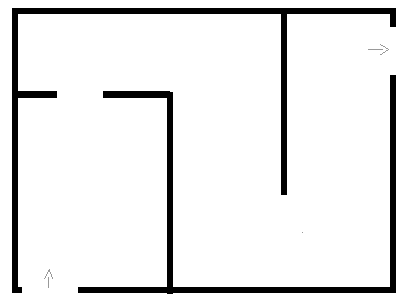
\includegraphics[keepaspectratio = true,
					width=1.0\textwidth]{img/missao3.png}
					\caption{Missão 3: Trajeto completo num ambiente com obstáculos}
					\label{fig:missao3}
				\end{figure}
			\end{column}
		\end{columns}
			
			
\end{frame}	


\section{Conclusão}

\begin{frame}
	\frametitle{Sumário}
	\tableofcontents[currentsection]
\end{frame}

\begin{frame}
	
	\frametitle{Conclusão}
	
	\begin{itemize}	
		
		\item  Enfoque em um tema surgente e relevante
		
		\item Inúmeras aplicações na área de defesa
		
		\item Construção do módulo de desvio de obstáculos da plataforma VANT-IME 
		
		
	\end{itemize}	
	
	
\end{frame}	


% -------------------------------------------------%
% -------------------------------------------------%
\section*{Referências}

%\begin{frame}
%	\frametitle{Sumário}
%	\tableofcontents[currentsection]
%\end{frame}

%\setbeamertemplate{bibliography item}[text]
\begin{frame}[allowframebreaks]{Bibliography}
	\frametitle{\insertsection}
	\bibliographystyle{abbrv}
	\footnotesize\bibliography{Dissertacao}
\end{frame}


% -------------------------------------------------%


\section*{Obrigado}
\begin{frame}[b]
	\frametitle{}
	
	
  	\centering{\textbf{Obrigado}
  	\\
  	\vspace{0.5cm} \footnotesize{ bsgiovanini@gmail.com} \\
	}
	\vspace{2cm}
	\hfill
	\begin{columns}[T]
		\begin{column}[T]{3cm}	
	
			
\includegraphics[height=1.0cm,keepaspectratio]{img/ime.jpg}\centering
		\end{column}
		\begin{column}[T]{3cm}
	
			
\includegraphics[height=1.0cm,keepaspectratio]{img/lab-logo.png}\centering
	
		\end{column}
	\end{columns}
		
	

\end{frame}



% -------------------------------------------------%
\end{document}